\documentclass[12pt]{article}                                                                                           
\usepackage{jmlda}
\usepackage{slashbox}

\title
    {Исследование изменения пространства параметров при дообучении и модификации моделей глубокого обучения}

\author
    {Иванов И.С., Бахтеев О.Ю.$^1$, Стрижов В.В.$^2$}
\thanks{$^1$консультант\newline$^2$научный руководитель и постановщик задачи}

\abstract{
    Статья посвящена задаче выбора оптимальной модели классификации временных рядов с использованием глубокого обучения.
    Рассматривается суперпозиция моделей, относящихся к следующим классам нейронных сетей: автокодировщики и двухслойные нейронные сети. 
    Предлагается исследовать дисперсию и матрицу ковариаций параметров модели при различных подходах к поэтапному обучению, на основе чего предложить эффективный способ модификации модели глубокого обучения.
    
\bigskip
\textbf{Ключевые слова}: \emph{выбор модели классификации; пространство параметров; дисперсия; ковариационная матрица; нейронные сети глубокого обучения}.
}

\begin{document}\maketitle
\section{1. Введение}
В данной работе рассматривается задача выбора и оптимизации модели классификации временных рядов. Под временным рядом понимается упорядоченный набор измерений некоторой величины, в котором каждое измерение соответствует определенному моменту времени. Исходная модель описана в статье \cite{Popova}. Модель использует нейронные сети глубокого обучения для выделения информативных признаков и классификации временных рядов. Она представляет собой многоуровневую суперпозицию автокодировщиков \cite{autoencoder} и двухслойных нейронных сетей \cite{two-layer-nn}. Все уровни суперпозиции, кроме последнего, обучаются по принципу «обучение без учителя» и участвуют в построении признакового пространства. Последний уровень суперпозиции обучается «с учителем» и решает задачу классификации по признакам, выделенным на нижних уровнях суперпозиции.

Предобучением называется предварительное обучение модели по принципу «обучение без учителя». Предобучение \cite{pre-train} слоев модели помогает избавиться от шумов во временных рядах и выделить необходимые признаки, тем самым стабилизируя параметры модели для дальнейшего дообучения (обучения всей сети по принципу «обучение с учителем»). Для поиска оптимальной модификации модели исследуется дисперсия и матрица ковариаций параметров нейросети на разных уровнях при различных подходах к поэтапному обучению. Строится add-del метод (метод добавления/удаления признаков) \cite{add-del} по полученным данным. Проблемой данного анализа является большой размер ковариационных матриц.

Проблема выбора оптимальной модели является достаточно изученной \cite{on-optim, tune, predict}. Существуют различные методы оптимизации нейронной сети, в том числе такие техники прореживания сети, как Optimal Brain Damage \cite{OBD} и Optimal Brain Surgeon \cite{OBS}. Для оптимизации гиперпараметров используют алгоритмы случайного поиска и некоторые жадные алгоритмы \cite{hyper-param, rand-hyper-param}. При рассмотрении нейронных сетей как вероятностных моделей \cite{prob-model}, применяются байевские методы оптимизации \cite{bayes}.

В данной работе поставлен вычислительный эксперимент на двух выборках -- временных рядах акселерометра и временных рядах акселерометра и гироскопа мобильного телефона.

\section{2. Постановка задачи}
Дана выборка $\mathfrak{D} =\left\{ (\mathbf{x}_i, \mathbf{t}_i) \right\}, i\in\mathcal{I}=\{1 \dots m\}$, состоящая из~$m$ объектов, каждый~из~которых описывается~$n$ признаками~$\mathbf{x}_i\in\mathbb{R}^n$ и~принадлежит одному из~$z$ классов~$\mathbf{t}_i\in\{0,1\}^z$. Также задано~разбиение множество индексов выборки $\mathcal{I} = \mathcal{L}\sqcup \mathcal {T}$ на обучающую ${(\mathbf{x}_i,\mathbf{t}_i)}, i \in \mathcal{L}$ и контрольную ${(\mathbf{x}_i,\mathbf{t}_i)}, i \in \mathcal{T}$.~Требуется выбрать устойчивую модель классификации оптимальной сложности.
\begin{Def}
Моделью назовем отображение:
\begin{equation*}
\mathbf{f} : (\mathbf{w},\mathbf{X}) \mapsto \mathbf{y},
\end{equation*}
где $\mathbf{w} = [w_1, \dots,w_j,\dots,w_n]^{\T}, j \in \mathcal{J} = \{1,\dots, n\}$ --- вектор параметров модели, $\mathbf{X} \in \mathbb{R}^{n\times m}$~---~матрица плана, $\mathbf{y} \in \{0,1\}^z$ --- зависимая переменная.
\end{Def}

В данной работе  рассматриваются модели, представляющие собой многоуровневую суперпозицию автокодировщиков и двухслойных нейронных сетей c функциями активации $\tanh$  и softmax:
\begin{equation*}
\mathbf{a(\mathbf{x})} = \mathbf{W}_2^{\T}\mathbf{tanh}(\mathbf{W}_1^{\T}\mathbf{x}),
\end{equation*}
\begin{equation*}
\mathbf{p(\mathbf{x})} = \frac {\exp(\mathbf{a(\mathbf{x})})}{\sum_j \exp(a_j(\mathbf{x}))}.
\end{equation*}
Вектор~$\mathbf{p}$ интерпретируется как вектор вероятностей: $p_{\xi}$ есть вероятность того, что вектор $\mathbf{x}$ принадлежит классу с номером ${\xi}$:
\begin{equation*}
\mathbf{p(\mathbf{x})} = \{p_\xi\},\quad 0 \leq p_{\xi} \leq 1,\quad \sum p_{\xi} = 1, \quad {\xi} = 1\dots z.
\end{equation*}
Под вектором параметров модели будем понимать  $\mathbf{w} = \text{vec}(\mathbf{W}_1^{\T}|...|\mathbf{W}_2^{\T})$, где $\mathbf{W}_i$~---~матрица весов~i-го~слоя~нейронной~сети. Вектор~$\mathbf{y}=[y_1,\dots,y_{\xi},\dots,y_z]^{\T}$ определим следующим образом:
\begin{equation*}
y_{\xi} = \begin{cases}
1, & \mbox{если}~{\xi} = \mathop{\text{argmax}}\limits_{\xi \in \{1,\dots,z\}} (p_{\xi}),  \\
0, & \mbox{иначе}.
\end{cases}
\end{equation*}
Под структурными параметрами модели будем понимать количество нейронов во внутренних слоях автокодировщиков и двухслойных нейронных сетей --- $N_i$.
\begin{Def}
Параметр $w_j$ модели $\mathbf{f}$ назовем активным, если $w_j \neq 0$.
\end{Def}
\begin{Def}
Структурой $\mathcal{A}$ модели $\mathbf{f}$ назовем множество индексов активных параметров этой модели $\mathcal{A} = \{j: w_j \neq 0 \} \subseteq \mathcal{J}$.
\end{Def}
Каждая структура $\mathcal{A} \subseteq \mathcal{J}$ однозначно задает некоторую модель:
\begin{equation*}
\mathbf{f}_{\mathcal{A}} : \mathbf{\hat{w}}_{\mathcal{A}} \in \mathbb{R}^n,
\end{equation*}
где $\mathbf{f}_{\mathcal{A}}$ --- модель со структурой $\mathcal{A}$, а $\mathbf{\hat{w}}_{\mathcal{A}} \in \mathbb{R}^n$ --- оптимальный вектор параметров модели $\mathbf{f}_{\mathcal{A}}$, определение которому будет дано ниже. Объединение всех $\mathbf{f}_\mathcal{A}$ назовем множеством допустимых моделей:
\begin{equation}
\label{eq:2}
\mathfrak{F} = \bigcup\limits_{{\mathcal{A} \subseteq \mathcal{J}}}\{\mathbf{f}_\mathcal{A}\}.
\end{equation}
Оптимальную модель $\mathbf{\hat{f}}_{\mathcal{A}}$ будем выбирать из множества допустимых моделей~$\mathfrak{F}$.

В качестве функции ошибки выберем функцию:
\begin{equation}
\label{eq:3}
S(\mathbf{w}|\mathcal{K}) = - \sum_{i \in \mathcal{K}} \sum_{\xi = 1}^{z} t_{i{\xi}}\ln \bigl( p_{\xi}(\mathbf{x}_i, \mathbf{w}) \bigr),
\end{equation}
максимизирующую логарифм правдоподобия случайной величины $\mathbf{y}$ и заданную на разбиении выборки $\mathfrak{D}$, определенном некоторым множеством индексов $\mathcal{K} \subseteq \mathcal{I}$, $\mathbf{t}_i = [t_{i1},\dots,t_{i\xi},\dots,t_{iz}]^{\T}$.
\begin{Def}
Оптимальным вектором параметров модели $\mathbf{f}_{\mathcal{A}}$  назовем такой вектор~$\mathbf{\hat{w}}_{\mathcal{A}}$, который является решением следующей задачи оптимизации:
\begin{equation}
\label{eq:4}
\mathbf{\hat{w}}_{\mathcal{A}} = \mathop{\text{argmin}}\limits_{{\mathbf{w}_{\mathcal{A}} \in \mathbb{R}^k}}S(\mathbf{w}_\mathcal{A}|\mathcal{L}).
\end{equation}
\end{Def}
Для оценки качества моделей и сравнения их друг с другом введём два критерия качества --- устойчивость и точность.
\begin{Def}
Устойчивостью $\eta = \eta(\mathbf{\hat{w}})$~модели $\mathbf{f}$ c вектором параметров $\mathbf{w}$ назовем число $\eta$, равное числу обусловленности матрицы ковариаций \textbf{Cov}($\mathbf{w}$), т.е. $\eta(\mathbf{\hat{w}})=\frac{\lambda_{\max}}{\lambda_{\min}}$, где $\lambda_{\max}$ --- максимальное, а $\lambda_{\min}$ --- минимальное собственное число матрицы \textbf{Cov}($\mathbf{w}$).
\end{Def}
Чем лучше обусловлена матрица \textbf{Cov}($\mathbf{w}$), тем более устойчива модель. У идеально устойчивой модели $\lambda_{\min} = \lambda_{\max},~\eta = 1$.
\begin{Def}
Под точностью $S$ модели $\mathbf{f}$ с вектором параметров $\mathbf{\hat{w}}$ будем понимать величину, обратную функции ошибки (\ref{eq:3}) на контрольной выборке.
\end{Def}
Чем больше значение функции ошибки, тем меньше точность модели. Задача выбора оптимальной модели состоит~в~том,~чтобы~найти модель, имеющую максимальную точность, из множества допустимых моделей $\mathfrak{F}$.

\section{3. Стратегия жадной модификации модели}
Наша стратегия модификация модели задается следующими математическими объектами:
\begin{itemize}
\item критериями устойчивости $\eta$ и точности $S$,
\item набором ограничений на структуру и параметры модели~$\mathcal{A} \subseteq \mathcal{J}$,~$\mathbf{w} = \mathbf{\hat{w}}_{\mathcal{A}}$ из ($\ref{eq:4}$),
\item критерием устойчивого прореживания~($\ref{eq:9}$).
\end{itemize}
Действуя согласно стратегии, мы будем изменять структуру модели, удаляя из неё элементы. Для определения индекса параметра $\hat{j}$, который должен быть удален из модели, предлагается следующий критерий оптимизации модели.

\subsection{3.1 Критерий устойчивого прореживания}
Критерий устойчивого прореживания основан на модификации метода Белсли и оценке ковариационной матрицы параметров.

Пусть $\mathbf{W}$  --- матрица реализаций оптимального вектора параметров~$\mathbf{\hat{w}}$, определенного~в~($\ref{eq:4}$). Пусть эта матрица имеет размерность $r \times k$. По реализациям вектора параметров вычисляется выборочная матрица ковариаций - \textbf{Cov}($\mathbf{w}$). Предполагается, что она блочно-диагональный вид, где блоки образованы нейронами (входящими в них весовыми функциями). При этом близость элемента матрицы к нулю трактуется как независимость соответствующих параметров.

Оценками дисперсии параметров будут диагональные элементы \textbf{Cov}($\mathbf{w}$):
\begin{equation*}
\sigma(w_{\zeta}) = \textbf{Cov}(\mathbf{w})_{\zeta \zeta}.
\end{equation*}

Выполним сингулярное разложение \textbf{Cov}($\mathbf{w}$):
\begin{equation}
\label{eq:8}
\textbf{Cov(w)} = \mathbf{U}\mathbf{S}\mathbf{V}^{\T},
\end{equation}
где $\mathbf{U}$ и $\mathbf{V}$ --- ортогональные матрицы размера $r \times r$ и $k \times k$ соответственно, а $\mathbf{\Lambda}$ --- матрица, на диагонали которой стоят сингулярные числа матрицы \text{cov}($\mathbf{w}$).

Индексом обусловленности $\eta_{\zeta}$ назовём отношение максимального элемента $\lambda_{\max}$ матрицы $\mathbf{\Lambda}$ к ${\zeta}$-ому по величине элементу $\lambda_{\zeta}$ этой матрицы:
\begin{equation*}
\eta_{\zeta} = \frac{\lambda_{\max}}{\lambda_{\zeta}}.
\end{equation*}

Долевой коэффицент $q_{{\zeta}j}$ определим как вклад $j$-го признака в дисперсию ${\zeta}$-го элемента вектора параметров $\mathbf{w}$:
\begin{equation*}
q_{{\zeta}j} = \frac {u_{{\zeta}j}^2\lambda_{jj}^2}{\sigma(w_{\zeta})}.
\end{equation*}

Найдём индексы обусловленности и долевые коэффициенты для набора активных параметров $\mathcal{A}$. Большие значения индексов обусловленности указывают на зависимость между признаками. Поэтому для нахождения параметра, отвечающего этому критерию прореживания, находим максимальный индекс обусловленности:
\begin{equation*}
\hat{{\zeta}} = \mathop{\text{argmax}}\limits_{{{\zeta} \in \mathcal{A}}}\eta_{\zeta}.
\end{equation*}
Затем находим максимальный долевой коэффициент, соответствующий найденному максимальному индексу обусловленности $\eta_{\hat{{\zeta}}}$:
\begin{equation}
\label{eq:9}
\hat{j} = \mathop{\text{argmax}}\limits_{{j \in \mathcal{A}}}q_{\hat{{\zeta}}j},
\end{equation}
Параметр $w_{\hat{j}}$ и есть параметр, отвечющий критерию устойчивого прореживания.

\subsection{3.2 Описание базовой стратегии}
Стратегия жадной модификации модели состоит из последовательности этапов Del.

\textbf{Этап Del.} Во множестве активных параметров ищем параметр с индексом $\hat{j}$, отвечающий критерию прореживания~($\ref{eq:9}$) и удаляем его из множества активных параметров:
\begin{equation*}
\mathcal{A} = \mathcal{A} \backslash \hat{j}.
\end{equation*}

Сперва модель предобучается, приобретая вектор параметров $\mathbf{w}_{0}$. После этого она независимо дообучается l раз, приобретая вектора параметров $\mathbf{w}_{1},...,\mathbf{w}_{l}$, на основе которых мы и вычисляем выборочную ковариационную матрицу. Далее повторяем этап Del некоторое заданное число раз, исключая параметры из вектора $\mathbf{w}_{0}$. После чего остается дообучить модель с модифицированным пространством параметров и измерить её качество.

\section{4. Вычислительный эксперимент}
В вычислительном эксперименте использовался набор временных рядов с акселерометра мобильного устройства -- WISDM \cite{Kwapisz2010Activity}. Цель вычислительного эксперимента заключалась в проверке эффективности предложенной стратегии модификации модели и сравнения полученных результатов с другими методами.
% подробнее про методы
\subsection{4.1 Программное обеспечение}
Эксперимент производился на ПО \cite{bah-code}, предназначенном для создания, обучения и оценки моделей глубокого обучения.
% подробнее про фреймворк
\subsection{4.2 Эксперимент}
Набор состоял из сегментов временных рядов акселерометра мобильного телефона, каждый из которых описывал один из четырех типов физической активности человека -- ходьбу, бег, стояние и сидение. Сегмент представлял из себя 10 секундный отрезок исходного временного ряда и состоял из 600 измерений -- по 200 измерений проекции ускорения на каждую из координатных осей. С более подробным описанием данных можно ознакомиться в работе \cite{Kwapisz2010Activity}.

Сбалансированная выборка состояла из 12546 объектов. В эксперименте использовалась трёхслойная суперпозиция, состоящая из двух автокодировщиков и однослойной нейросети с нелинейной функцией активации с 200, 6 и 6 нейронами в каждом слое соответственно. Автокодировщики предобучались на 1000 объектах. Дообучение реализовывалось в рамках кросс-валидации на оставшихся 11546 объектах, разделение на обучающую и контрольную выборку проводилось случайным образом в соотношении 3:1. Было произведено 15 итераций кросс-валидации, на основе изменений вектора параметров были посчитаны дисперсии компонент вектора, гистограммы для параметров первых двух слоёв изображены на рис.~$\ref{fg:1}$.

\begin{figure}[!h]
%  \centering
  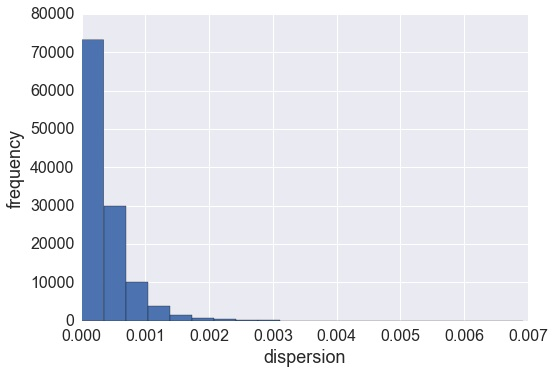
\includegraphics[width=0.5\textwidth]{disp1.jpg}{}
  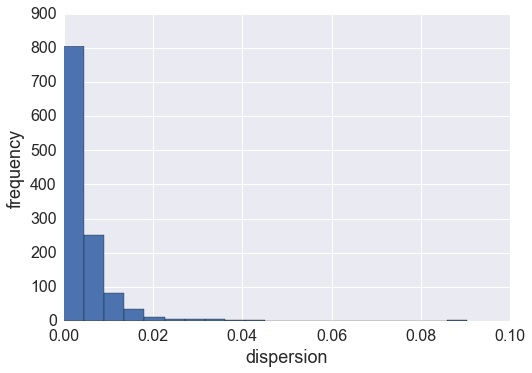
\includegraphics[width=0.5\textwidth]{disp2.jpg}{}
  \caption{Распределение дисперсий весовых функций по слоям}
  \label{fg:1}
\end{figure}

Далее измерялось влияние удаления (обнуления) части параметров сети на качество работы модели. В эксперименте удалялось от 10 до 70 процентов всех параметров. Для сравнения качества работы модели измерялась точность модели при классификации тестовой выборки. Предложенным методом выбора параметров на удаление является модифицированный метод Белсли, описанный в разделе 3.1. Для сравнения также были проведены эксперименты с другими методами. Из предположения, что неустойчивые (имеющие большую дисперсию) параметры могут оказывать наименьшее влияние на модель, в одном из экспериментов удалялись параметры с наибольшей дисперсией. В остальных экспериментах к удалению были отобраны параметры с наименьшей дисперсией и случайно выбранные параметры. Результаты измерений изображены на рис.~$\ref{fg:2}$.

\begin{figure}[!h]
%  \centering
  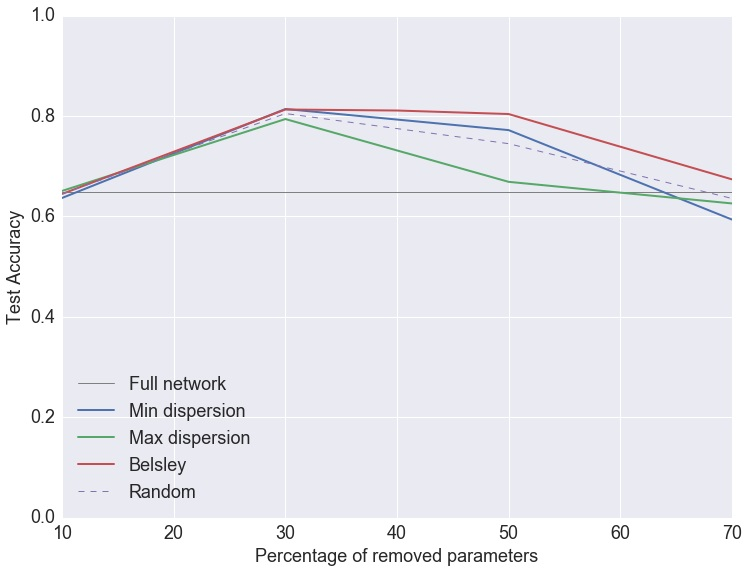
\includegraphics[width=1.0\textwidth]{graph.jpg}{}
  \caption{Зависимость точности модели от процента отброшенных параметров}
  \label{fg:2}
\end{figure}

Из графика видно, что при помощи модификации модели удалось увеличить её точность. При этом предложенный метод показал лучшие результаты.

\section{4. Заключение}
В данной работе рассмотрена задача классификации временных рядов при помощи глубокой нейронной сети. Исследовано влияние различных методов разряжения пространства параметров на качество модели глубокого обучения. Предлагаемый метод, основанный на методе Белсли, показал относительно хороший результат и, имея теоретические обоснования, может быть использован в других задачах.

В дальнейшем планируется проанализировать работу метода при пошаговой модификации.

\begin{thebibliography}{1}

\bibitem{Zadayanchuk}
    \BibAuthor{Задаянчук А.\,И., Попова М.\,С., Стрижов В.\,В.}
    \BibTitle{Выбор оптимальной модели классификации физической активности по измерениям акселерометра}
    \BibUrl{http://strijov.com/papers/Zadayanchuk2015OptimalNN4.pdf}
\bibitem{Popova}
    \BibAuthor{Попова М.\,С., Стрижов В.\,В.}
    \BibTitle{Построение сетей глубокого обучения для классификации временных рядов}
    \BibUrl{http://strijov.com/papers/PopovaStrijov2015DeepLearning.pdf}
\bibitem{Bahteev}
    \BibAuthor{Бахтеев О.\,Ю., Попова М.\,С., Стрижов В.\,В.}
    \BibTitle{Системы и средства глубокого обучения в задачах классификации}
    \BibUrl{http://svn.code.sf.net/p/mlalgorithms/code/Group074/Bakhteev2015TheanoCuda/doc/Bakhteev2015TheanoAWS.pdf}
\bibitem{Popova}
    \BibAuthor{Попова М.\,С., Стрижов В.\,В.}
    \BibTitle{Выбор оптимальной модели классификации физической активности по измерениям акселерометра}
    \BibUrl{http://svn.code.sf.net/p/mlalgorithms/code/Group174/Popova2014OptimalModelSelection/doc/Popova2014OptimalModelSelection.pdf}
\bibitem{OBD}
    \BibAuthor{LeCun Y.}
    \BibTitle{Optimal Brain Damage}
    \BibUrl{http://yann.lecun.com/exdb/publis/pdf/lecun-90b.pdf}
\bibitem{pre-train}
    \BibAuthor{Dumitru Erhan, Yoshua Bengio, Aaron Courville, Pierre-Antoine Manzagol, Pascal Vincent, Samy Bengio}
    \BibTitle{Why Does Unsupervised Pre-training Help Deep Learning?}
    \BibJournal{Journal of Machine Learning Research 11 (2010) 625-660}
    \BibUrl{http://jmlr.org/papers/volume11/erhan10a/erhan10a.pdf}
\bibitem{autoencoder}
    \BibAuthor{Andrew Ng}
    \BibTitle{Sparse autoencoder}
    \BibJournal{CS294A Lecture notes}
    \BibUrl{https://web.stanford.edu/class/cs294a/sparseAutoencoder.pdf}
\bibitem{add-del}
    \BibAuthor{Воронцов К.В.}
    \BibTitle{Оценивание моделей и отбор признаков}
    \BibUrl{http://www.machinelearning.ru/wiki/images/archive/4/4f/20111004204412!Voron-ML-Modeling-slides.pdf}
\bibitem{hyper-param}
    \BibAuthor{James Bergstra, Remi Bardenet, Yoshua Bengio, Balazs Kegl}
    \BibTitle{Algorithms for Hyper-Parameter Optimization}
    \BibUrl{http://papers.nips.cc/paper/4443-algorithms-for-hyper-parameter-optimization.pdf}
\bibitem{rand-hyper-param}
    \BibAuthor{James Bergstra, Yoshua Bengio}
    \BibTitle{Random Search for Hyper-Parameter Optimization}
    \BibJournal{Journal of Machine Learning Research 13 (2012) 281-305}
    \BibUrl{http://www.jmlr.org/papers/volume13/bergstra12a/bergstra12a.pdf}
\bibitem{prob-model}
    \BibAuthor{David J.C. MacKay}
    \BibTitle{Bayesian Methods for Neural Networks: Theory and Applications}
    \BibUrl{http://www.inference.eng.cam.ac.uk/mackay/cpi4.pdf}
\bibitem{bayes}
    \BibAuthor{Yarin Gal, Zoubin Ghahramani}
    \BibTitle{Dropout as a Bayesian Approximation: Insights and Applications}
    \BibUrl{http://mlg.eng.cam.ac.uk/yarin/PDFs/Dropout_as_a_Bayesian_approximation.pdf}
\bibitem{info-theory}
    \BibAuthor{Naftali Tishby, Noga Zaslavsky}
    \BibTitle{“Optimal Deep Learning” and the Information Bottleneck method}
    \BibJournal{ICRI-CI retreat, Haifa, May 2015}
    \BibUrl{http://icri-ci.technion.ac.il/files/2015/05/01-Tali-Tishby-1505051.pdf}
\bibitem{two-layer-nn}
    \BibAuthor{G. Brightwell, C. Kenyon, H. Paugam-Moisy}
    \BibTitle{Multilayer neural networks: one or two hidden layers?}
    \BibUrl{http://papers.nips.cc/paper/1239-multilayer-neural-networks-one-or-two-hidden-layers.pdf}
\bibitem{OBS}
    \BibAuthor{Babak Hassibi, David G. Stork, Gregory J Wolff}
    \BibTitle{Optimal Brain Surgeon and General Network Pruning}
    \BibUrl{http://ee.caltech.edu/Babak/pubs/conferences/00298572.pdf}
\bibitem{on-optim}
    \BibAuthor{Quoc V. Le, Jiquan Ngiam, Adam Coates, Abhik Lahiri, Bobby Prochnow, Andrew Y. Ng}
    \BibTitle{On Optimization Methods for Deep Learning}
    \BibUrl{http://machinelearning.wustl.edu/mlpapers/paper_files/ICML2011Le_210.pdf}
\bibitem{tune}
    \BibAuthor{M. Bashiri}
    \BibTitle{Tuning the parameters of an artificial neural network using central composite design and genetic algorithm}
    \BibUrl{http://www.sciencedirect.com/science/article/pii/S1026309811002136}
\bibitem{predict}
    \BibAuthor{Misha Denil, Babak Shakibi, Laurent Dinh, Marc’Aurelio Ranzato, Nando de Freitas}
    \BibTitle{Predicting Parameters in Deep Learning}
    \BibUrl{http://www.cs.toronto.edu/~ranzato/publications/denil_nips2013.pdf}
\bibitem{AnguitaGOPR1}
    \BibAuthor{Anguita D., Ghio A., Oneto L., Parra X., Luis Reyes-Ortiz J.} 
    \BibTitle{Human Activity Recognition on Smartphones Using a Multiclass Hardware-Friendly Support Vector Machine}
    \BibJournal{Ambient Assisted Living and Home Care: Proceedings of the 4th International Workshop (IWAAL 2012). --  Springer, 2012. Vol.\,7657. P.\,216--223}
\bibitem{Kwapisz2010Activity}
    \BibAuthor{Kwapisz\;J.\,R., Weiss\;G.\,M., Moore\;S.}
    \BibTitle{Activity recognition using cell phone accelerometers}
    \BibJournal{SIGKDD Explorations, 2010. Vol.\,12. No\,2. P.\,74--82}
\bibitem{bah-code}
    % \BibAuthor{Bahteev O.\,Y.}
    \BibTitle{Python-driven software for time-series classification}
    \BibUrl{http://svn.code.sf.net/p/mlalgorithms/code/Group074/Bakhteev2015Sysdocs}
    
\end{thebibliography}

\end{document}
